\chapter{实验结果与性能分析}


%*********************************************************************
% 5.1 全局指令选择正确性验证
%*********************************************************************
\section{全局指令选择正确性验证}


% 5.1.1 基本指令正确性验证
\subsection{基本指令正确性验证}
本节旨在验证DSP后端基本指令(除控制流指令及特殊指令之外的指令)的正确性,重点关注算术运算指令和内存访问指令的匹配和选择结果。为此本节设计了一个示例程序一,这个示例程序包含函数参数传递、内存读写操作和整数加法与乘法运算等操作,能够覆盖了DSP后端常见的指令选择路径。

\par

由于LLVM IR具有良好的目标无关性,且从C语言到LLVM IR的转换过程并非本文关注重点,本文在分析过程中省略前端生成IR的具体细节,直接展示从LLVM IR到目标机器码的转换流程,以突出指令选择与后端代码生成阶段的行为特征。


\subsubsection{1.LLVM IR输入}
示例程序一的LLVM IR如代码块\ref{lst:case_1_ir}所示,该示例程序包含了基本的算术与访存操作,后文将以此为基础分析指令选择过程中中间表示的演化。为了便于展示,已去除掉代码中的调试信息。

\lstset{language=c++}
\begin{lstlisting}[language=C++, caption={示例程序一的LLVM IR表示}, label={lst:case_1_ir}]
define dso_local i32 @testArith(i32 noundef %a, i32 noundef %b) {
	entry:
	%a.addr = alloca i32
	%b.addr = alloca i32
	store i32 %a, ptr %a.addr
	store i32 %b, ptr %b.addr
	%0 = load i32, ptr %a.addr
	%1 = load i32, ptr %b.addr
	%add = add i32 %0, %1
	%2 = load i32, ptr %a.addr
	%mul = mul i32 %add, %2
	ret i32 %mul
}
\end{lstlisting}


\subsubsection{2.GMIR生成阶段}
如图\ref{fig:case_1_gmir_gen_dump}所示,在GMIR生成阶段,LLVM IR被转换为与目标架构无关的GMIR。从中间结果可以观察到:

\begin{itemize}
	\item 
	alloca被映射为COPY指令,函数参数通过COPY指令从物理寄存器拷贝到虚拟寄存器。
	
	\item
	load与store分别被映射为G\_LOAD与G\_STORE。
	
	\item
	add与mul分别被映射为G\_ADD与G\_MUL。
	
	\item 
	ret被映射为RET。
	
\end{itemize}

\begin{figure}[htbp]
	\centering
	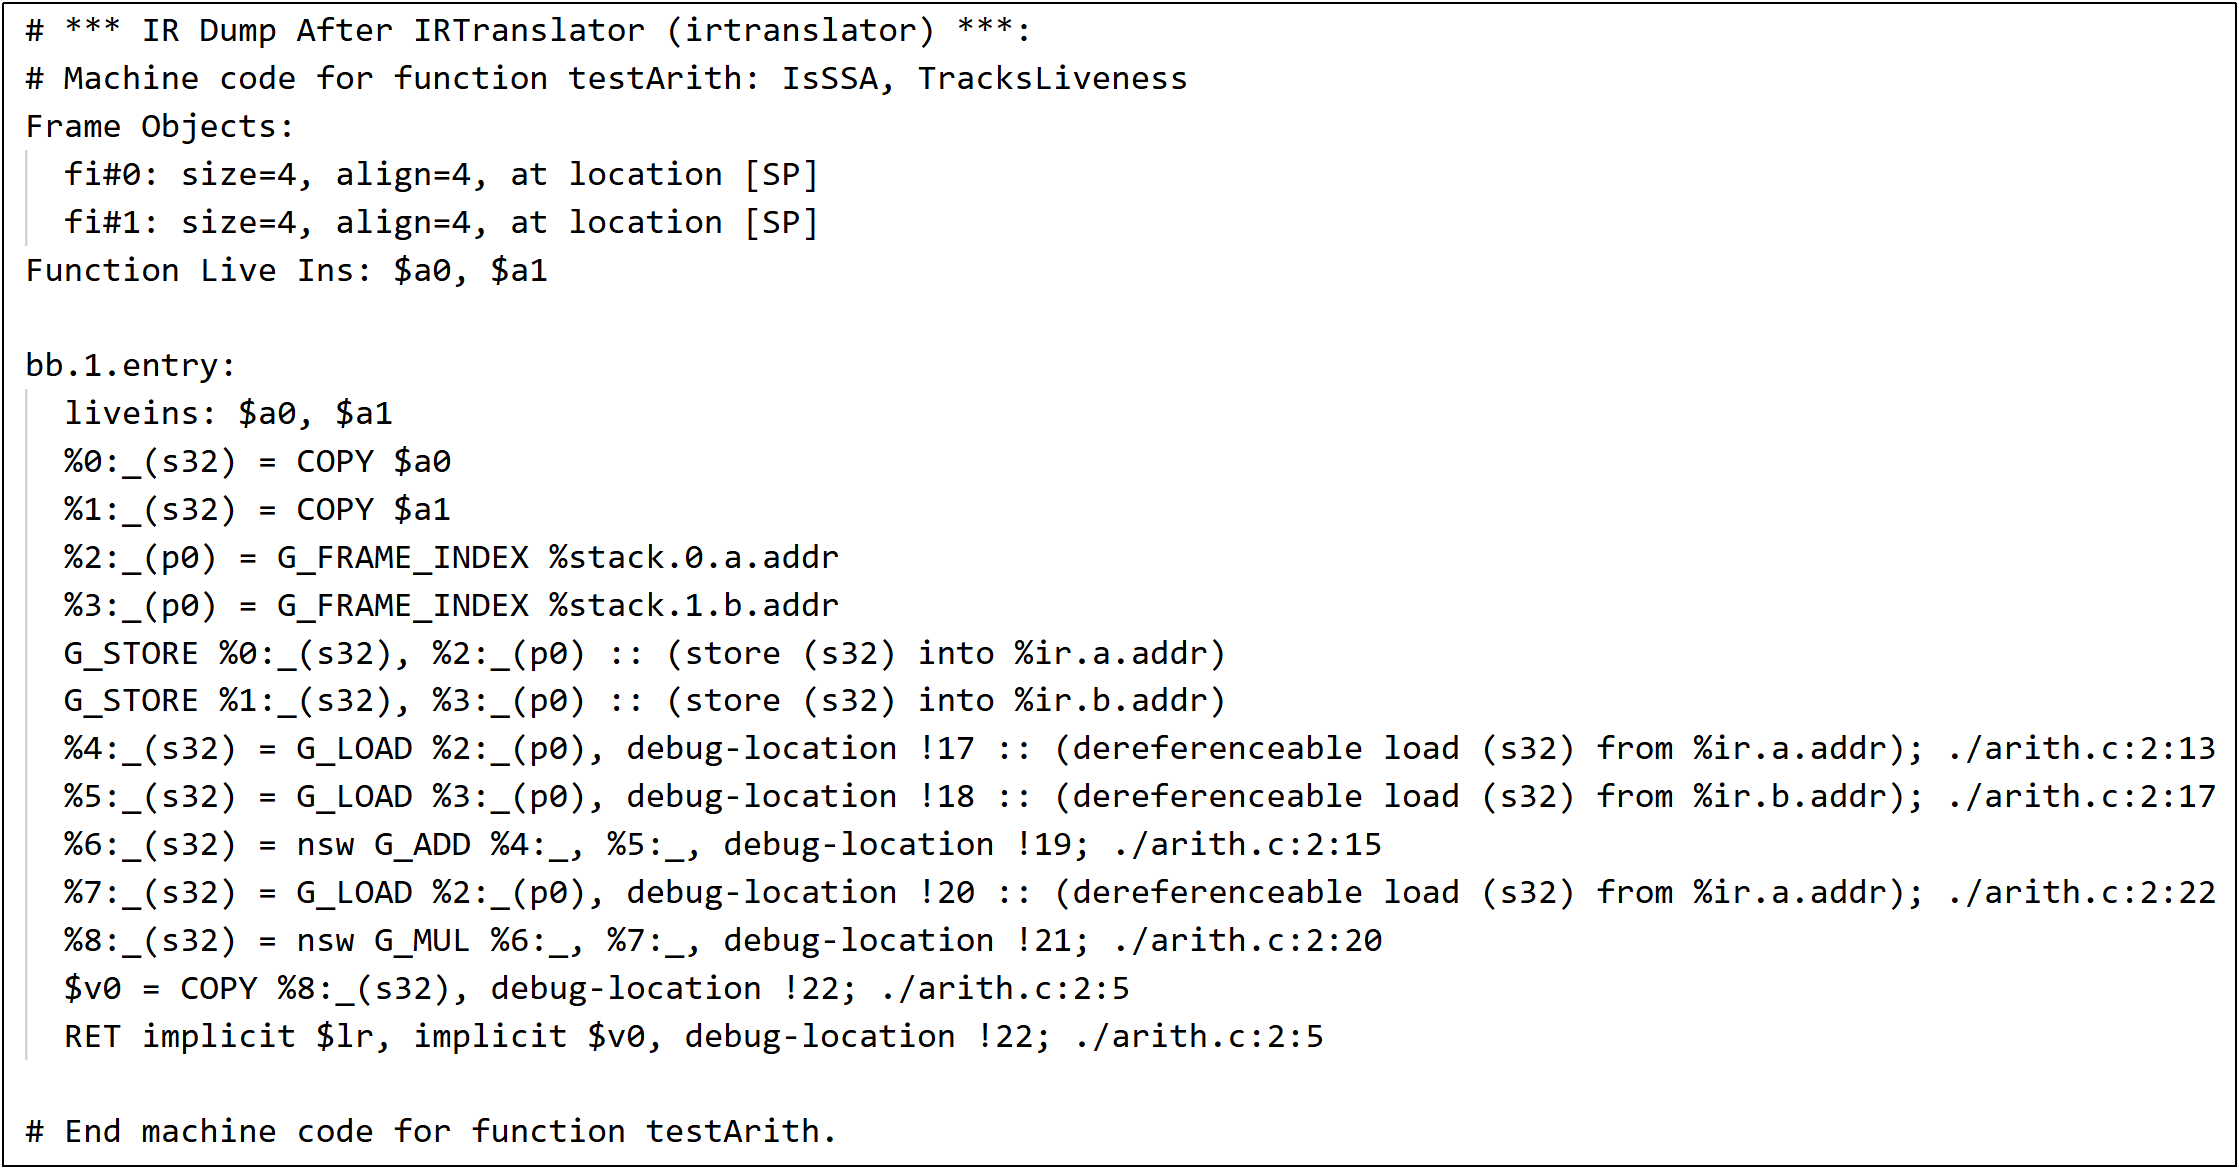
\includegraphics[width=1\textwidth]{pics/case_1_gmir_gen_dump.png}
	\caption{示例程序一的GMIR生成阶段Dump图}
	\label{fig:case_1_gmir_gen_dump}
\end{figure}

该结果表明,LLVM IR到GMIR的转换过程保持了原有运算语义与数据依赖关系,为后续后端处理提供了正确的输入。


\subsubsection{3.合法化阶段}
指令合法化阶段的核心任务,在于将GMIR中目标架构不直接支持的操作,转化为目标架构可以直接处理的合法形式。在本示例程序中,32位的G\_ADD、G\_MUL、G\_LOAD以及G\_STORE等指令均为DSP架构原生支持的操作,因此并未触发类型扩展及指令拆解等复杂的合法化过程。如图\ref{fig:case_1_legalize_dump}所示,合法化前后的指令序列在结构和语义上保持一致。这一结果表明,当前DSP合法化规则能够正确处理基本的算术运算与内存访问指令。

\begin{figure}[htbp]
	\centering
	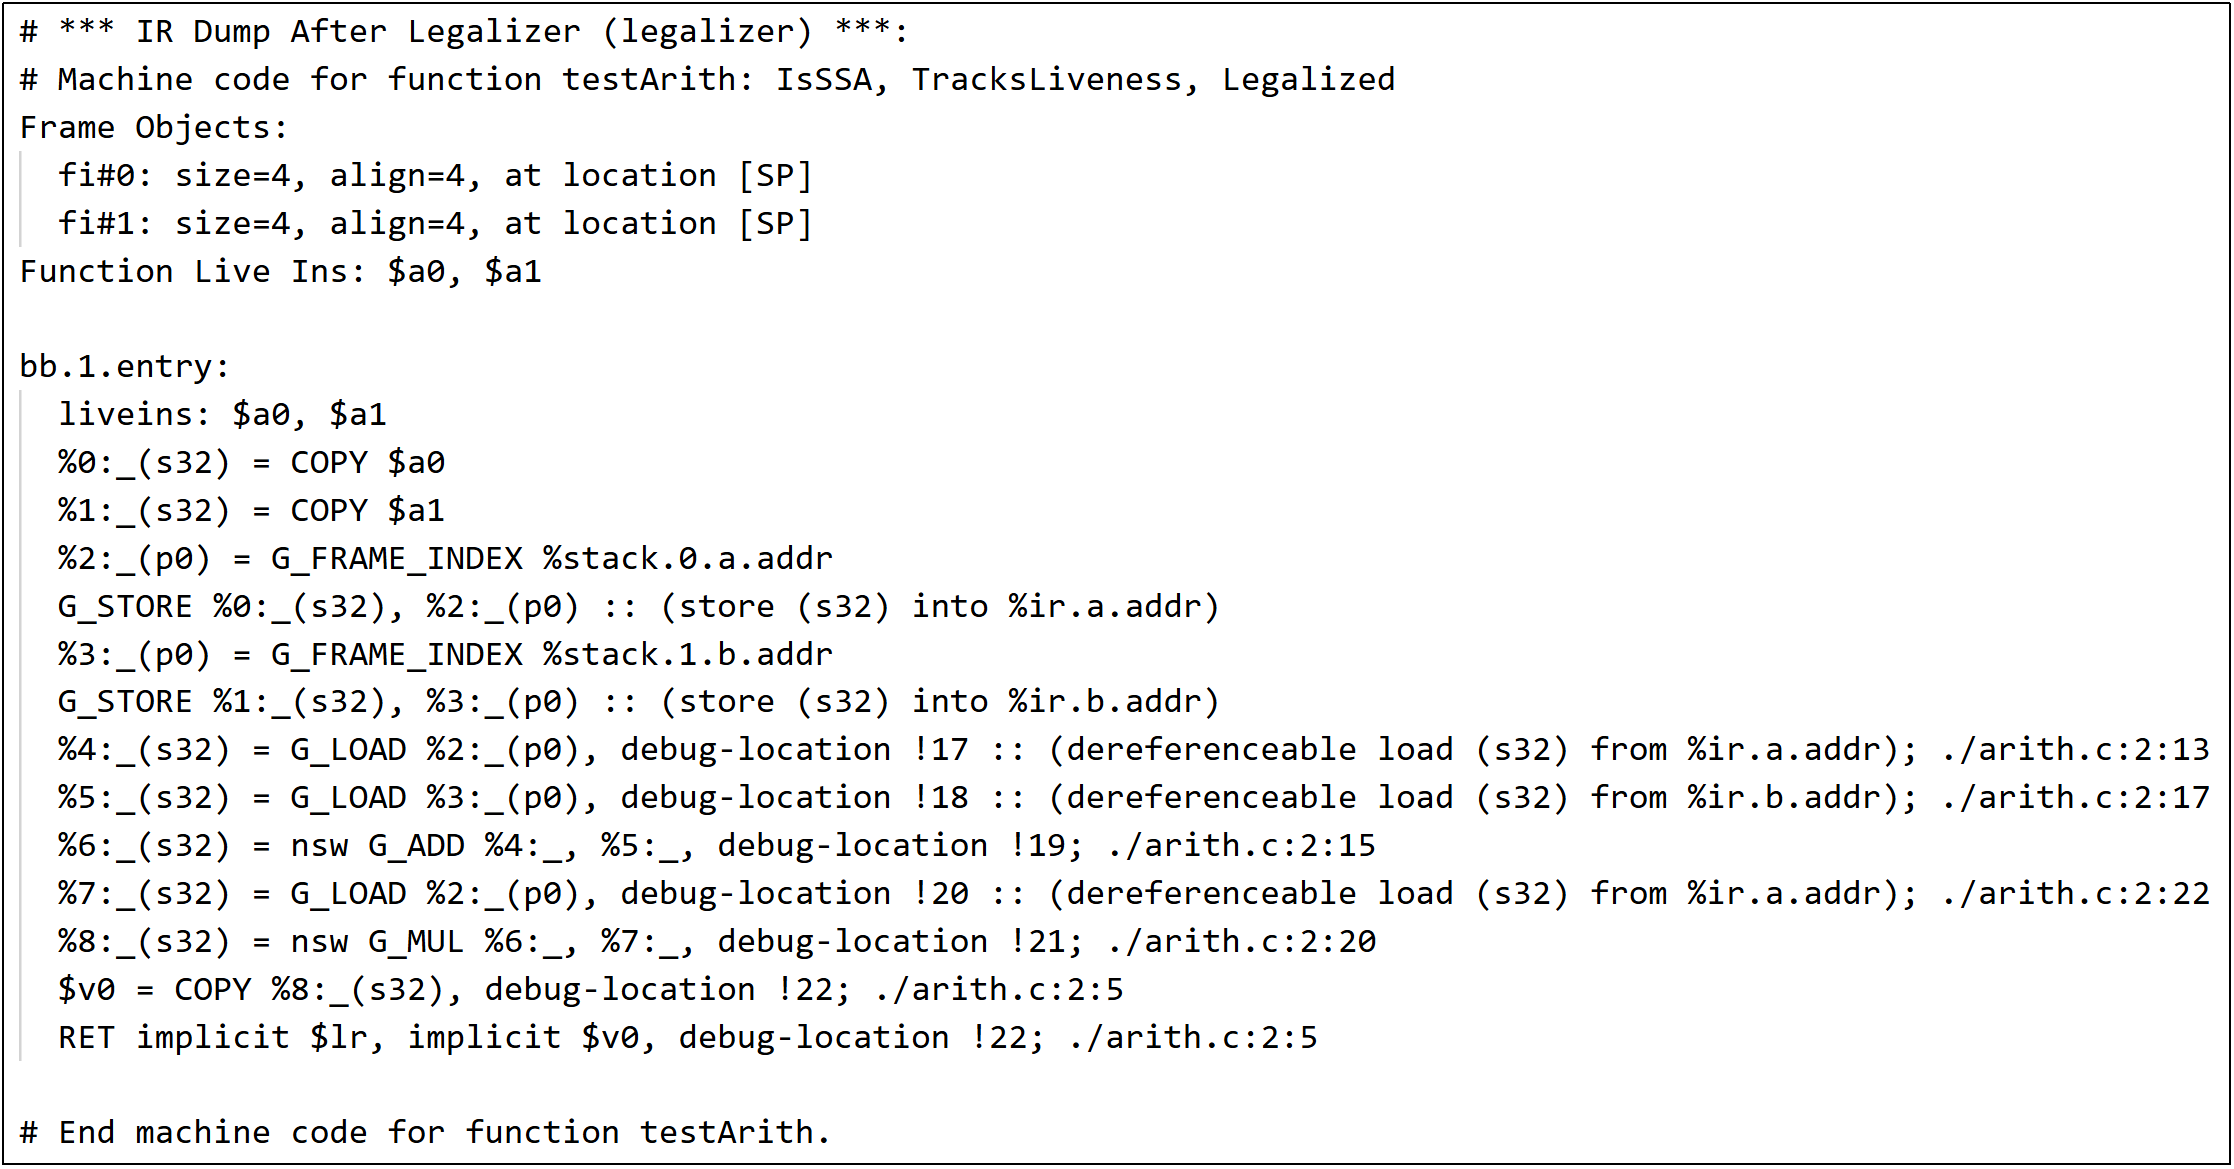
\includegraphics[width=1\textwidth]{pics/case_1_legalize_dump.png}
	\caption{示例程序一的合法化阶段Dump图}
	\label{fig:case_1_legalize_dump}
\end{figure}


\subsubsection{4.寄存器组选择阶段}
在寄存器组选择阶段,编译器需要为每个虚拟寄存器分配合适的寄存器组。在当前的DSP后端实现中,所有参与整数算术运算的虚拟寄存器都被统一映射至GPRB中。如图\ref{fig:case_1_regbank_select_dump}所示,从寄存器组选择后的中间结果可以观察到,所有算术指令的操作数及结果均被分配到GPRB寄存器组,并且寄存器类型与对应操作数的位宽保持一致,符合DSP架构对整数运算的寄存器使用约束。

\begin{figure}[htbp]
	\centering
	\includegraphics[width=1\textwidth]{pics/case_1_regbank_select_dump.png}
	\caption{示例程序一的寄存器组选择阶段Dump图}
	\label{fig:case_1_regbank_select_dump}
\end{figure}

该结果表明所有参与算术运算的虚拟寄存器均被正确分配至通用寄存器组,同时未引入额外的跨寄存器组数据复制或冗余中间指令。


\subsubsection{5.机器指令选择阶段}
在机器指令选择阶段,GMIR被转换为DSP架构的目标机器指令。如\ref{fig:case_1_instr_select_dump}所示,从中间结果可以观察到,除了COPY指令外的所有指令都被正确的映射到DSP后端机器指令,COPY指令需要在后续阶段中单独处理。

\begin{figure}[htbp]
	\centering
	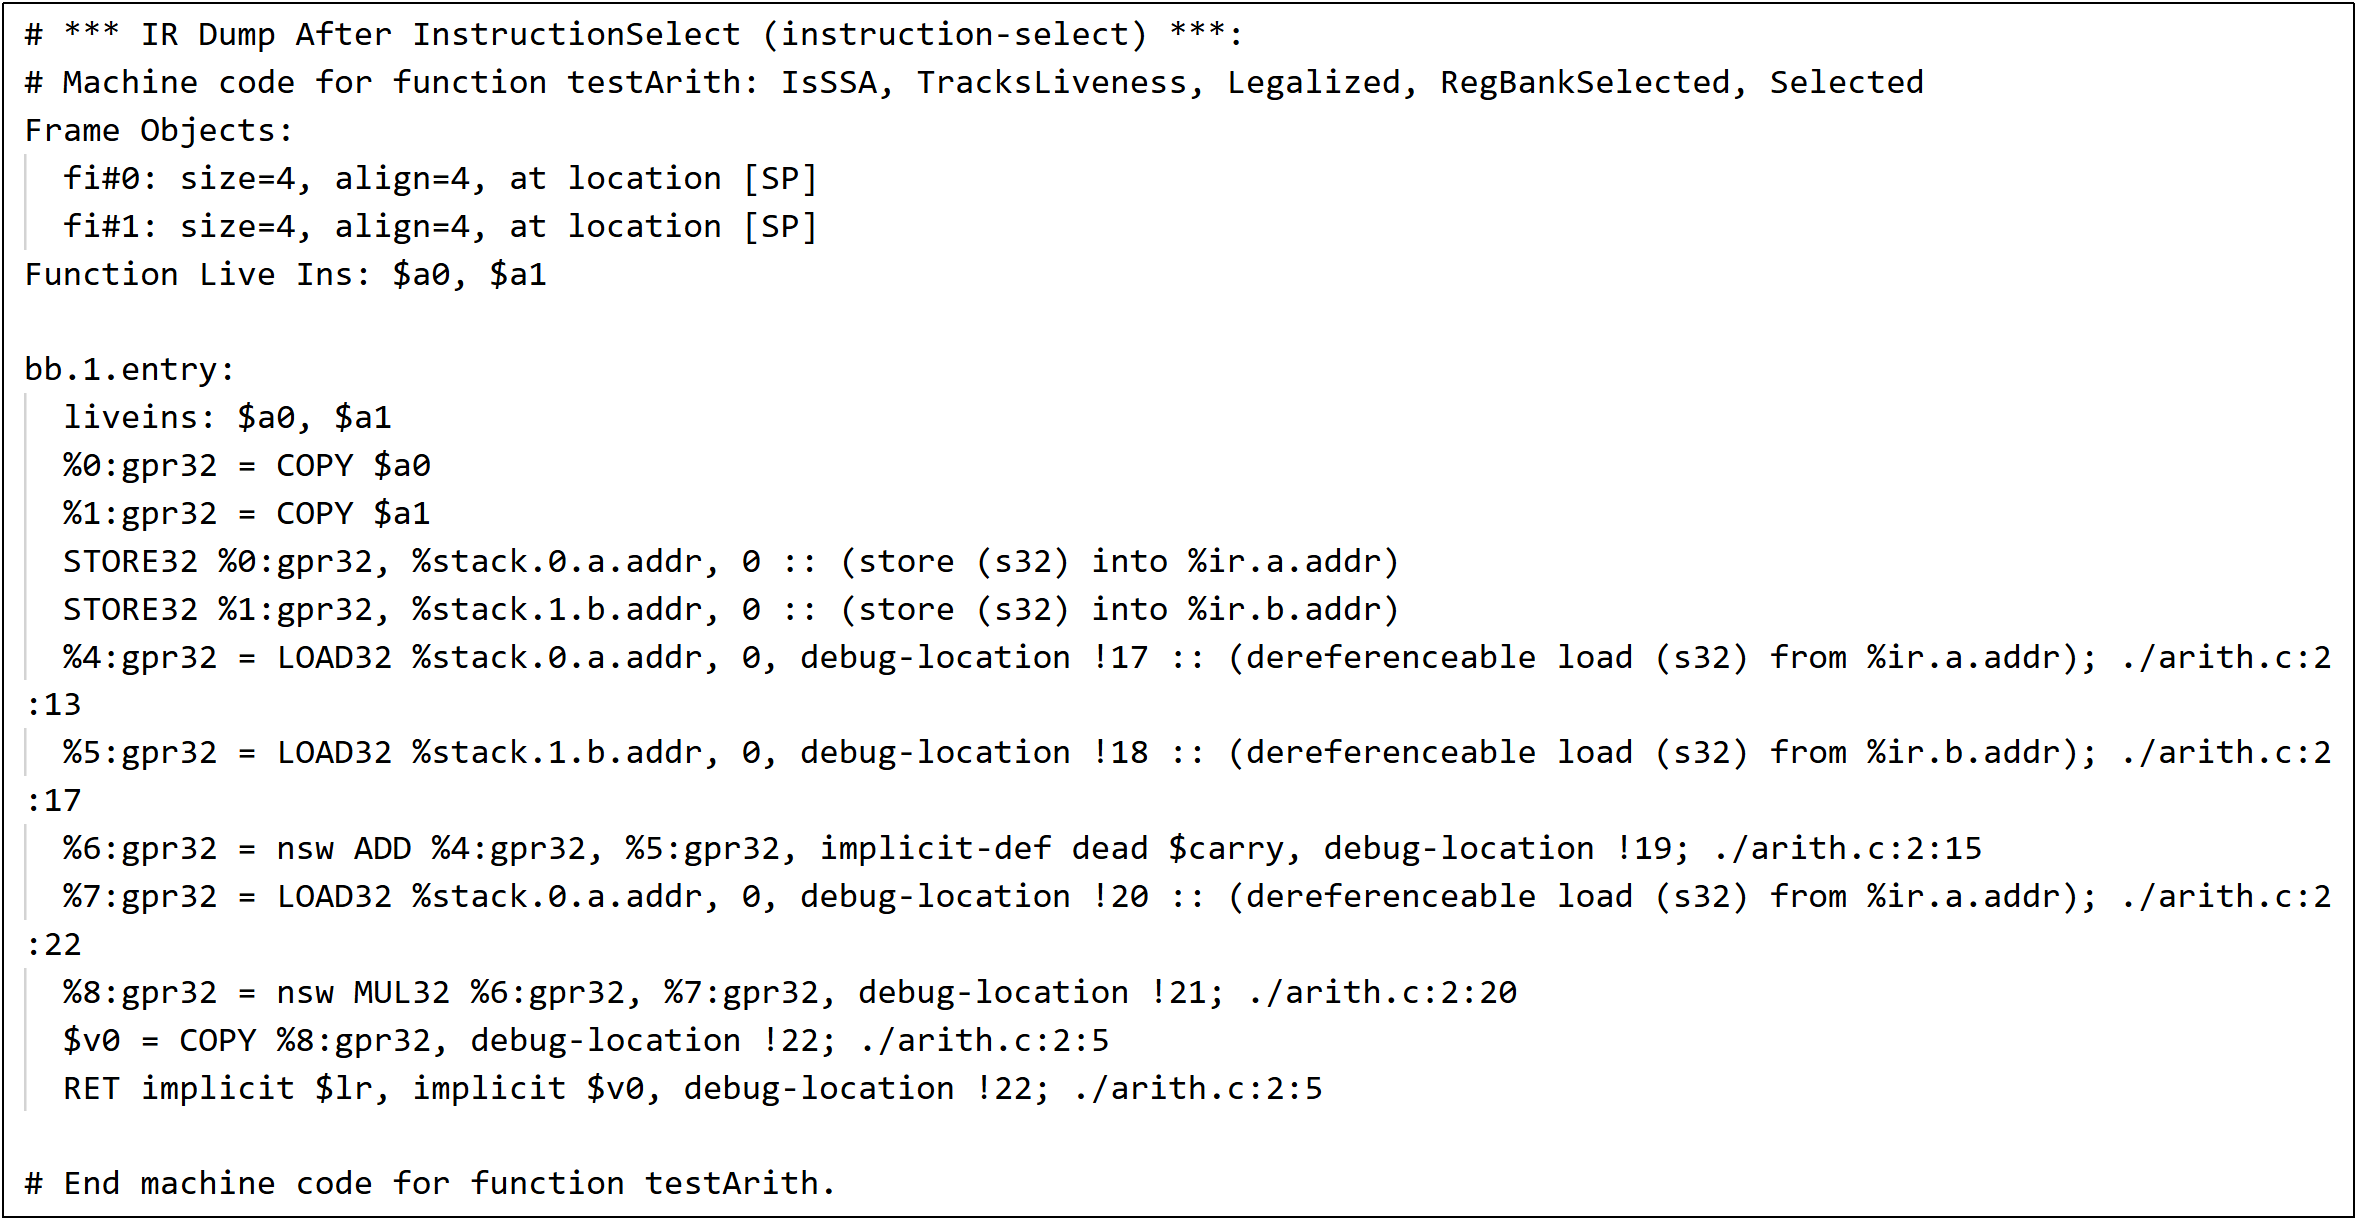
\includegraphics[width=1\textwidth]{pics/case_1_instr_select_dump.png}
	\caption{示例程序一的机器指令选择阶段Dump图}
	\label{fig:case_1_instr_select_dump}
\end{figure}


\subsubsection{6.最终代码生成阶段}
在完成寄存器分配以及指令调度等后续后端处理流程后,编译器最终生成了符合DSP指令集规范的目标代码。如图\ref{fig:case_1_final_dump}所示,生成的目标代码在指令顺序、操作数选择以及控制流结构等方面均与原始程序语义保持一致。这表明在该示例程序中,基于GlobalISel框架的代码生成流程能够在DSP后端上正确运行,实现了从高级LLVM IR到目标平台可执行机器指令的精准映射。

\begin{figure}[htbp]
	\centering
	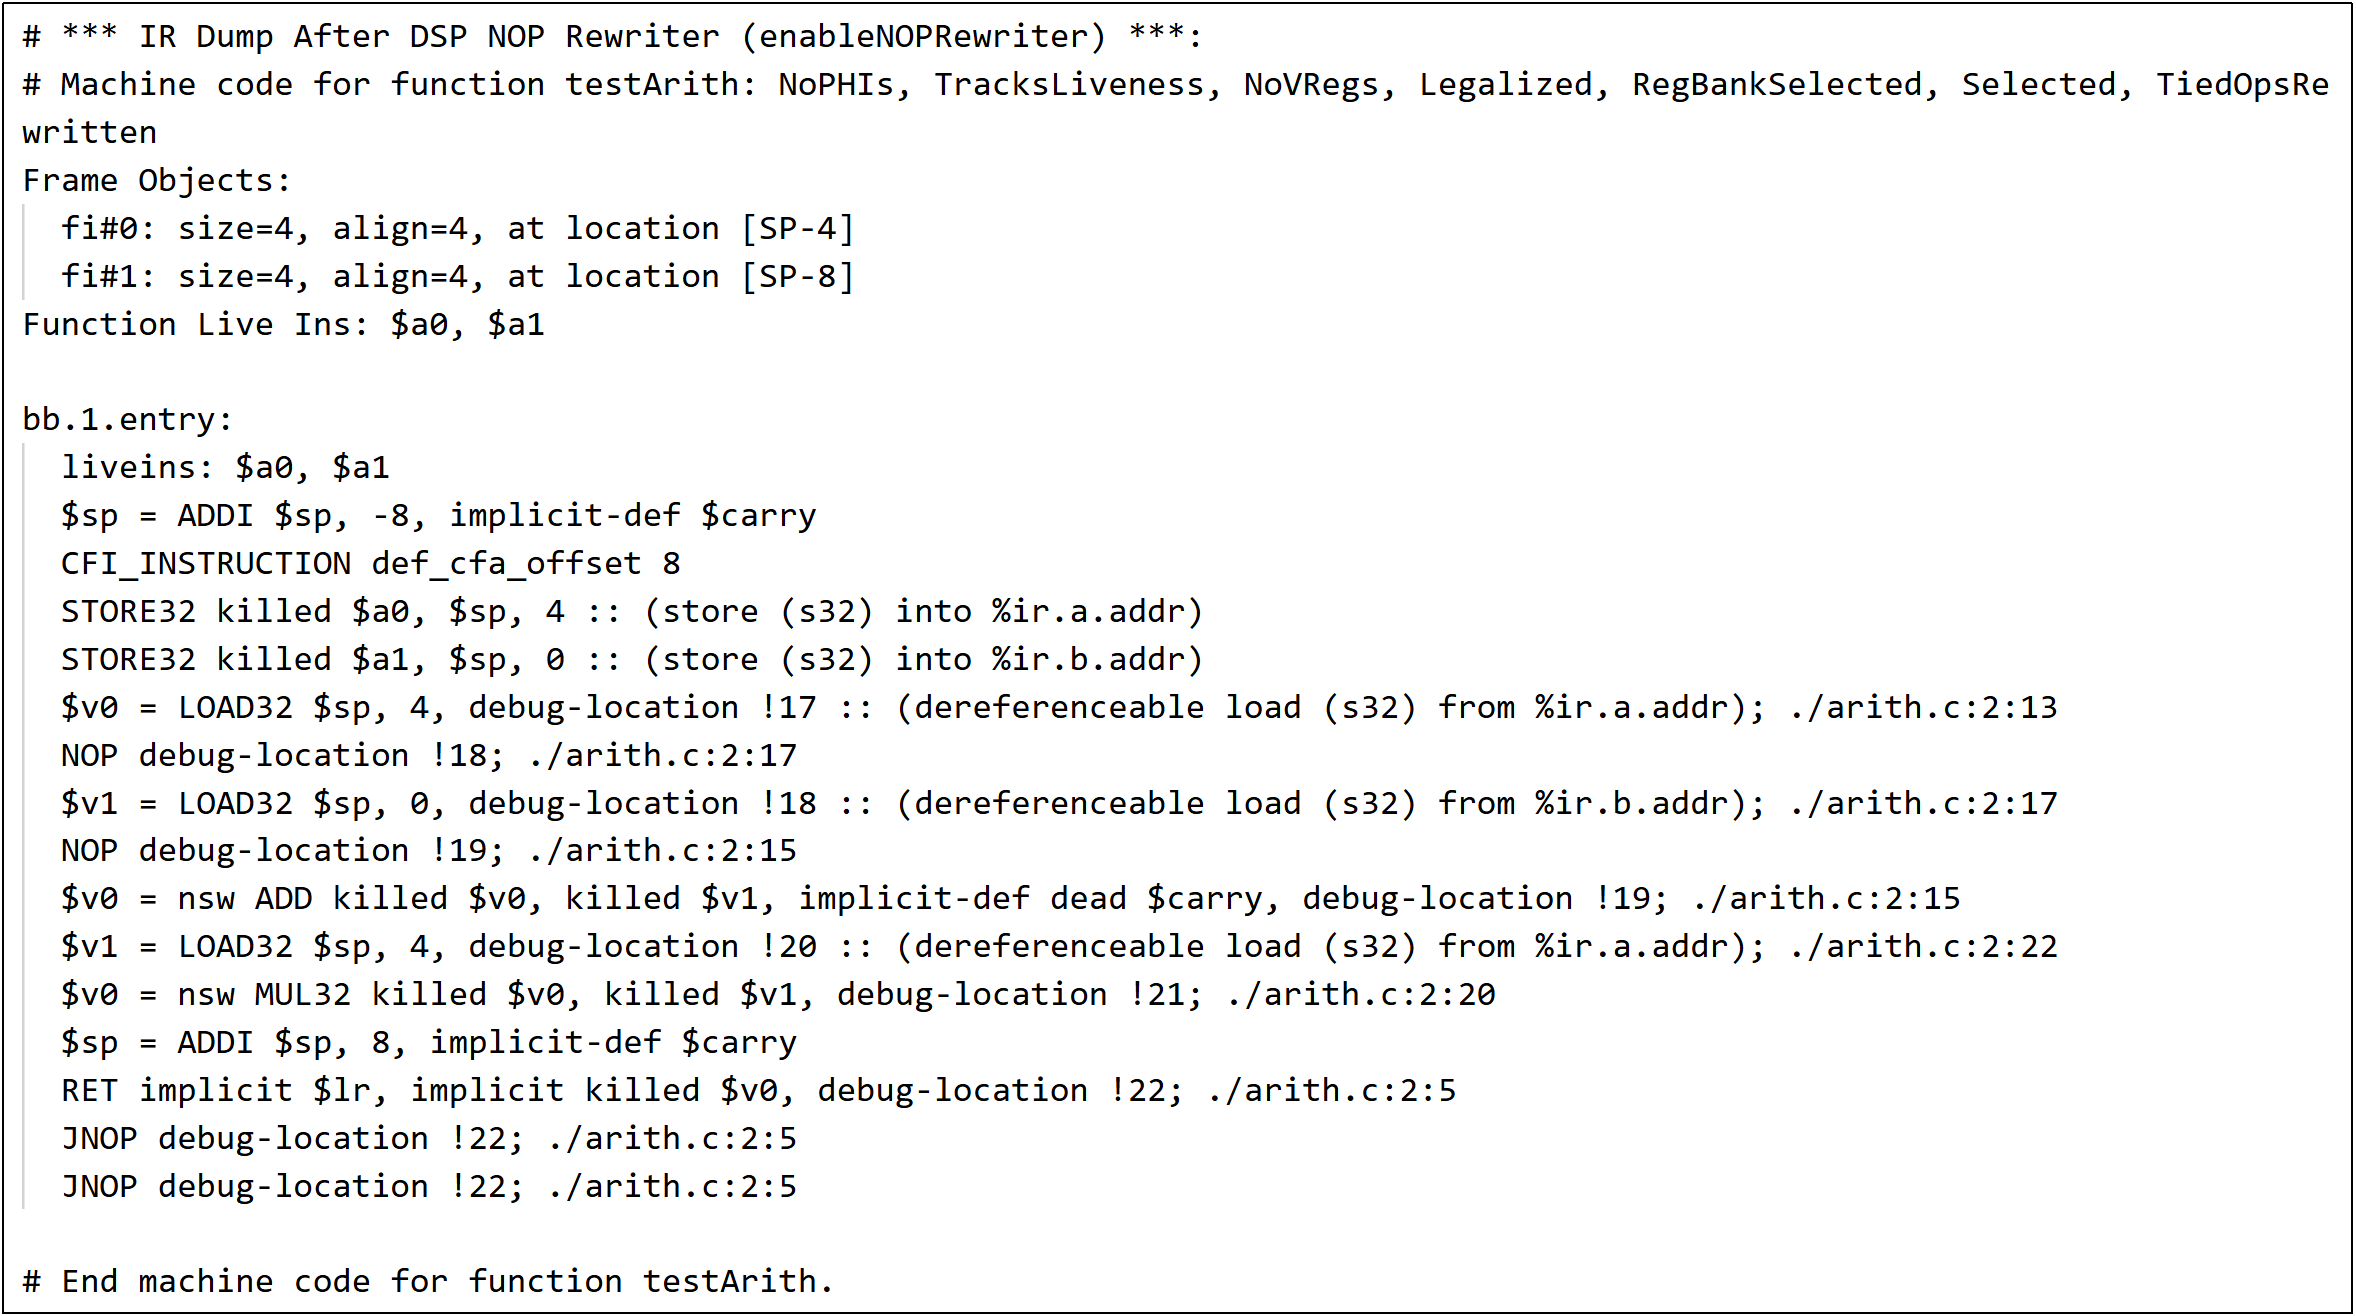
\includegraphics[width=1\textwidth]{pics/case_1_final_dump.png}
	\caption{示例程序一的最终阶段Dump图}
	\label{fig:case_1_final_dump}
\end{figure}


% 5.1.2 控制流指令正确性验证
\subsection{控制流指令正确性验证}
除基本算术与内存访问指令这些基本指令外,控制流指令的正确生成和映射同样是验证编译器后端正确性的重要体现。本节针对对控制流相关指令的处理过程进行验证,重点覆盖比较与条件分支、循环结构以及函数调用三类典型控制流场景。


\subsubsection{1.比较+分支+跳转指令}
比较与条件分支是程序控制流构建的基础。在LLVM IR中,比较与条件分支通过icmp与br组合表达。为验证DSP后端对该类控制流指令的处理正确性,本节构建了一个同时包含比较、条件分支及无条件跳转的示例程序二,其LLVM IR如代码块\ref{lst:case_2_ir}所示。

\lstset{language=c++}
\begin{lstlisting}[language=C++, caption={示例程序二的LLVM IR表示}, label={lst:case_2_ir}]
define dso_local i32 @testBranch() {
	entry:
	%retval = alloca i32
	%a = alloca i32
	%b = alloca i32
	store i32 10, ptr %a
	store i32 20, ptr %b
	%0 = load i32, ptr %a
	%1 = load i32, ptr %b
	%cmp = icmp slt i32 %0, %1
	br i1 %cmp, label %if.then, label %if.else
	
	if.then:
	store i32 0, ptr %retval
	br label %return
	
	if.else:
	store i32 1, ptr %retval
	br label %return
	
	return:  %2 = load i32, ptr %retval
	ret i32 %2
}
\end{lstlisting}

针对该示例程序,在GlobalISel各关键阶段中的处理过程如下:

\begin{itemize}
	\item
	在GMIR生成阶段,LLVM IR中的比较指令被正确转换为G\_ICMP,其比较谓词与操作数保持一致;条件跳转指令被转换为G\_BRCOND,并以比较结果作为分支条件。
	
	\item
	在合法化阶段,由于DSP架构支持整数比较操作,无需进一步拆分,相关指令保持原有结构。
	
	\item 
	在寄存器组选择阶段,编译器为比较操作及其结果所涉及的虚拟寄存器分配了合适的寄存器组,确保比较结果能够以符合DSP架构约定的方式参与后续控制流指令。
	
	\item 
	在机器指令选择阶段,G\_ICMP与后续的G\_BRCOND会被联合处理,映射为DSP架构下的比较指令与条件跳转指令,比较结果通过条件码寄存器传递,从而完成分支控制。
	
\end{itemize}

如图\ref{fig:case_2_final_dump}所示,在函数入口基本块中,比较指令首先生成条件码寄存器状态,随后通过条件跳转指令根据比较结果在两个后继基本块之间进行分支选择,验证了比较与条件分支指令的正确映射。

\begin{figure}[htbp]
	\centering
	\includegraphics[width=1\textwidth]{pics/case_2_final_dump.png}
	\caption{示例程序二入口基本块的最终阶段Dump图}
	\label{fig:case_2_final_dump}
\end{figure}

如图\ref{fig:case_2_final_dump_2}所示,条件判断成立时进入if.then基本块,不成立则进入if.else基本块,两个基本块各自执行相应的逻辑操作,且在块末尾均通过无条件跳转指令,汇合到同一个返回基本块中。从最终生成的机器码结果来看,各分支基本块间的跳转关系,以及这些分支块与返回块的连接方式,均与LLVM IR所定义的控制流结构一致,未产生任何额外的控制流变动。

\begin{figure}[htbp]
	\centering
	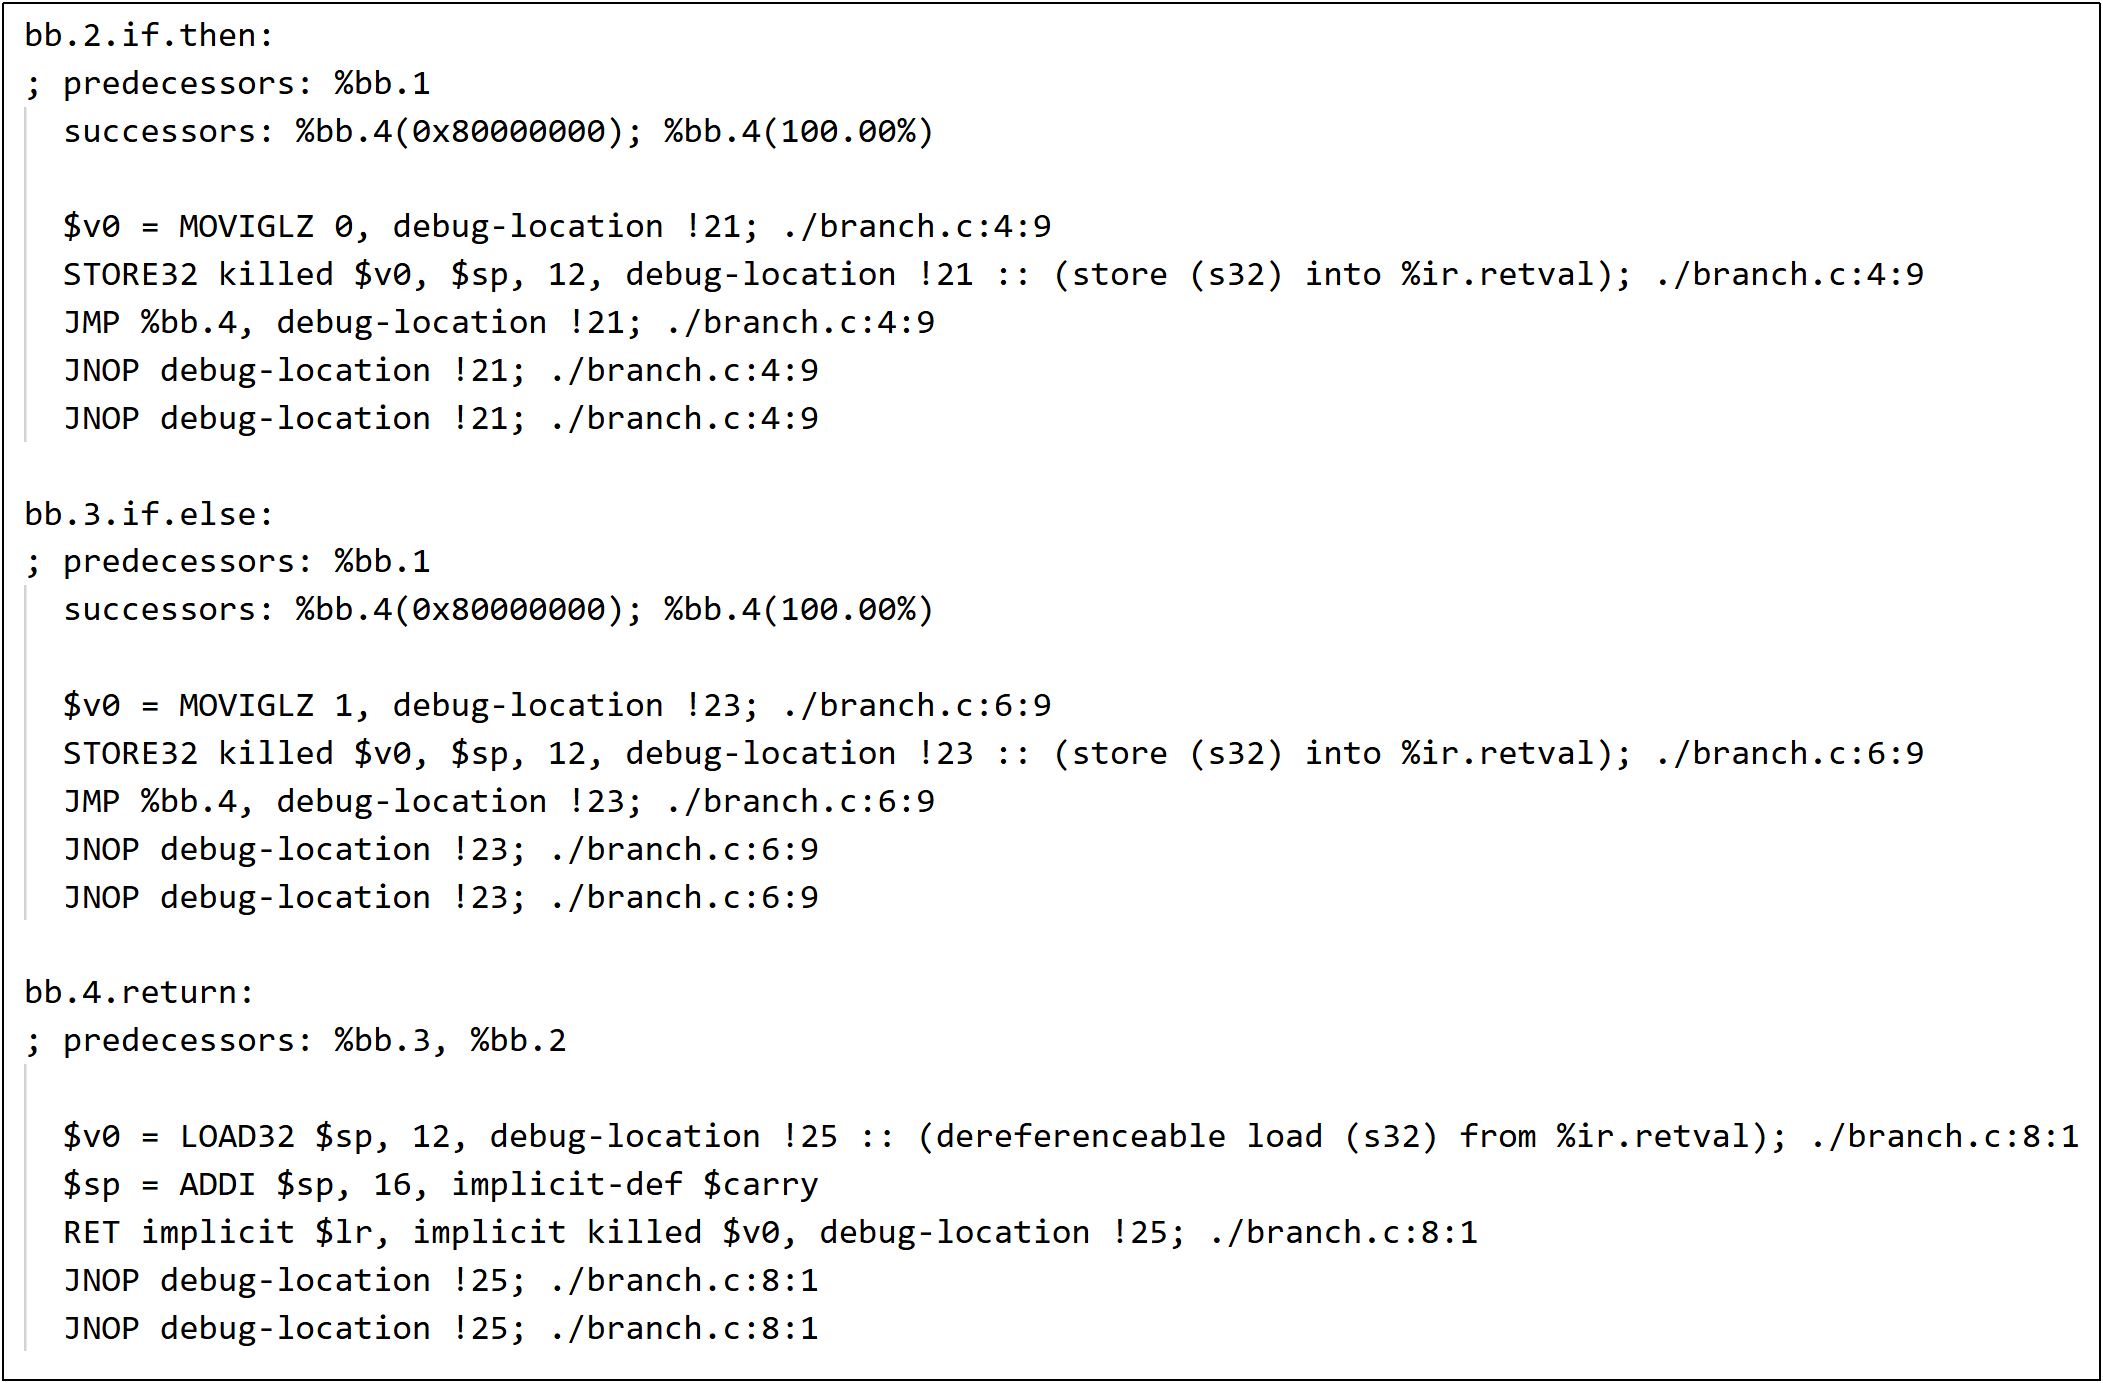
\includegraphics[width=1\textwidth]{pics/case_2_final_dump_2.png}
	\caption{示例程序二条件分支基本块的最终阶段Dump图}
	\label{fig:case_2_final_dump_2}
\end{figure}

从实验结果可以观察到,在LLVM IR向目标代码的转换过程中,比较条件及其对应的分支目标均保持一致,程序控制流未发生偏移或错误跳转,实验结果验证了比较、分支与跳转指令选择的正确性。


\subsubsection{2.循环指令}
在汇编语言层面,循环结构并没有像高级语言那样的专用语法结构,而是通过条件分支和跳转指令来实现。循环结构通常由条件判断、条件分支以及指向循环体起始的回边构成,在LLVM IR中,循环表现为由多个基本块及其间的br分支指令构成的子图。当LLVM IR被转换为GMIR时,这一多基本块结构及其控制流依赖关系被完整保留,从而为后端的指令选择与代码生成提供了清晰的控制流语义。

\par

为验证DSP后端对循环指令的处理正确性,本文构建了一个包含循环指令的示例程序三,其LLVM IR如代码块\ref{lst:case_3_ir}所示。

\lstset{language=c++}
\begin{lstlisting}[language=C++, caption={示例程序三的LLVM IR表示}, label={lst:case_3_ir}]
define dso_local i32 @testLoop() {
	entry:
	%i = alloca i32
	store i32 0, ptr %i
	br label %for.cond
	
	for.cond:
	%0 = load i32, ptr %i
	%cmp = icmp slt i32 %0, 10
	br i1 %cmp, label %for.body, label %for.end
	
	for.body:
	br label %for.inc, !dbg !21
	
	for.inc:
	%1 = load i32, ptr %i
	%inc = add nsw i32 %1, 1
	store i32 %inc, ptr %i
	br label %for.cond
	
	for.end:
	ret i32 0
}
\end{lstlisting}

针对该示例程序,在GlobalISel各关键阶段中的处理过程如下:

\begin{itemize}
	\item
	在GMIR生成阶段,各基本块及其控制流关系被准确映射为MBB,循环条件与跳转关系通过G\_BR与G\_BRCOND指令表达。
	
	\item
	在合法化阶段,合法化前后指令结构保持一致,表明DSP后端的合法化规则能够覆盖该类循环场景的基本操作需求。
	
	\item 
	在寄存器组选择阶段,循环体内的算术与内存操作被正确映射至DSP通用寄存器组,循环条件判断所依赖的比较结果亦能够被正确传播。
	
	\item 
	在机器指令选择阶段,循环控制流相关的G\_ICMP与G\_BRCOND被联合分析并映射为DSP架构下的比较指令与条件跳转指令:比较结果通过条件码寄存器生成,并由条件跳转指令读取实现分支决策。
	
\end{itemize}

如图\ref{fig:case_3_final_dump}所示,在循环条件基本块中,编译器首先将循环变量与上界进行比较,随后根据比较结果设置条件码寄存器,再借助条件码寄存器生成对应的分支条件,最后根据比较结果在循环体与循环结束块之间跳转。

\begin{figure}[htbp]
	\centering
	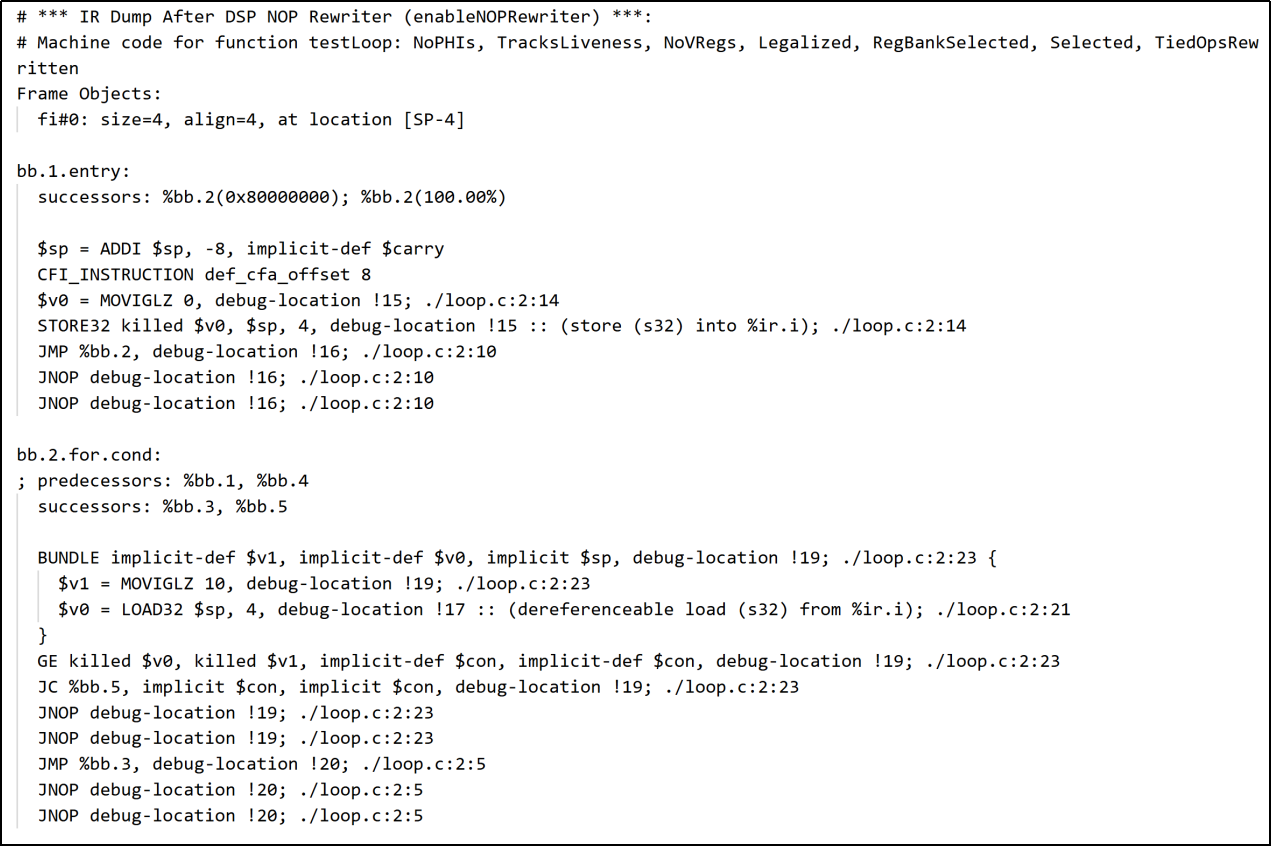
\includegraphics[width=1\textwidth]{pics/case_3_final_dump.png}
	\caption{示例程序三循环条件基本块的最终阶段Dump图}
	\label{fig:case_3_final_dump}
\end{figure}

如图\ref{fig:case_3_final_dump_2}所示,在循环体及其后续的自增操作基本块执行完毕后,程序通过一条无条件跳转指令形成回边,使控制流重新返回到循环条件判断块。当循环条件不再满足时,控制流则正确跳转至循环结束块,并最终执行函数返回。

\begin{figure}[htbp]
	\centering
	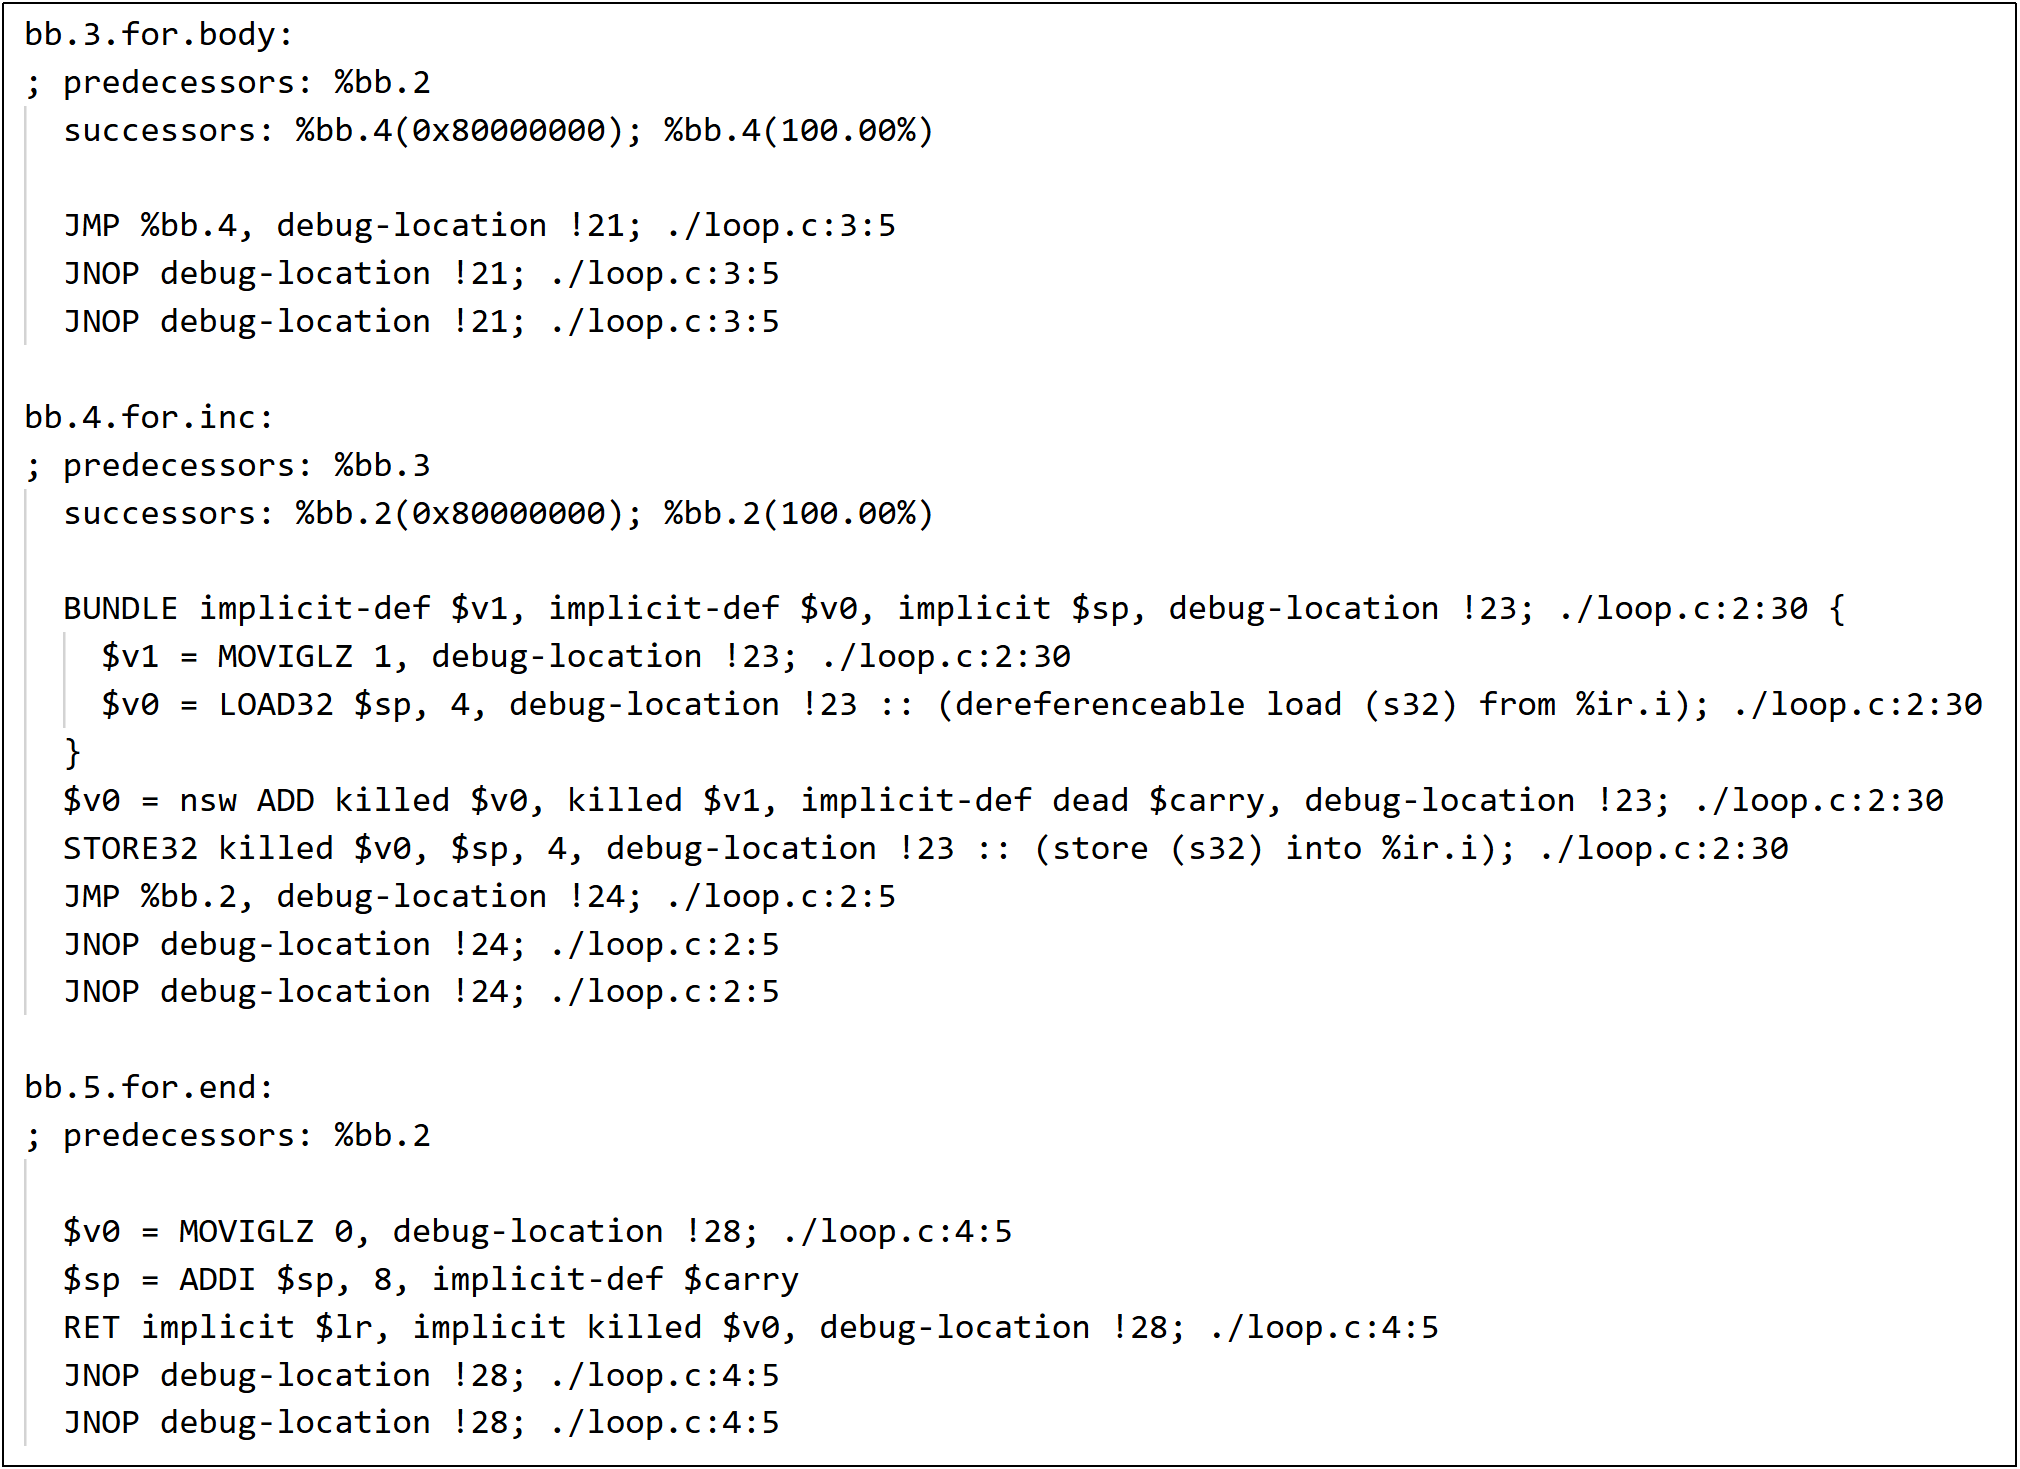
\includegraphics[width=1\textwidth]{pics/case_3_final_dump_2.png}
	\caption{示例程序三循环体基本块的最终阶段Dump图}
	\label{fig:case_3_final_dump_2}
\end{figure}

最终生成的目标代码表明,循环入口处的条件分支、循环体内部执行以及指向循环头的回边跳转,对应的指令序列均与原始LLVM IR所定义的控制流结构保持一致,且不存在冗余或缺失的跳转指令。这一结果说明GlobalISel在DSP后端中能够正确处理多基本块循环结构,保证循环语义的正确无误。


\subsubsection{3.函数调用指令}
函数调用也是一类重要的控制流操作,其正确性依赖于调用约定、参数传递机制以及返回值处理等多个环节。在LLVM IR中,函数调用通过call指令表示。在GlobalISel框架下,对函数调用的处理涵盖多个阶段,主要包括由CallLowering接口负责的调用规范lowering,以及后续在指令选择阶段对具体调用指令的匹配与生成。

\par

为验证DSP后端在GlobalISel框架下对函数调用指令的处理正确性,构造了一个简单的示例程序四,其中main函数调用前文定义的testBranch函数,其LLVM IR如代码块\ref{lst:case_4_ir}所示。

\lstset{language=c++}
\begin{lstlisting}[language=C++, caption={示例程序四的LLVM IR表示}, label={lst:case_4_ir}]
define dso_local i32 @main() {
	entry:
	%retval = alloca i32
	store i32 0, ptr %retval
	%call = call i32 @testBranch()
	ret i32 %call
}
\end{lstlisting}

针对该示例程序,函数调用在各阶段的处理过程如下:

\begin{itemize}
	\item
	在GMIR生成阶段,call指令被转换为与调用约定相关的一系列包括参数准备、调用指令以及返回值接收等操作的GMIR指令。
	
	\item
	在合法化阶段,合法化前后指令结构保持一致,表明DSP后端的合法化规则能够覆盖该类函数调用场景的基本操作需求。
	
	\item 
	在寄存器组选择阶段,函数参数与返回值在符合DSP ABI的规则下被分配至DSP架构规定的寄存器或栈位置。
	
	\item 
	在机器指令选择阶段,与调用相关的GMIR指令会被映射为DSP架构支持的跳转与返回指令。
	
\end{itemize}

如图\ref{fig:case_4_final_dump}所示,实验结果表明DSP后端在GlobalISel框架下能够正确完成函数调用相关控制流的指令选择,从而保证了跨函数控制流的正确传递。

\begin{figure}[htbp]
	\centering
	\includegraphics[width=1\textwidth]{pics/case_4_final_dump.png}
	\caption{示例程序四的最终阶段Dump图}
	\label{fig:case_4_final_dump}
\end{figure}


%*********************************************************************
% 5.2 全局指令选择性能分析
%*********************************************************************
\section{全局指令选择性能分析}
本章主要针对编译时间、代码大小以及执行周期三个方面来对基于DAG的指令选择、未优化的全局指令选择以及优化的全局指令选择来进行对比。


% 5.2.1 编译时间
\subsection{编译时间}
编译时间作为一项关键的工程指标,直接反映了编译器的可用性与开发迭代效率,尤其在需要持续进行性能优化与回归测试的编译器开发实践中,后端编译阶段的耗时变化将对整体开发效率产生显著影响。为此,本节将从编译时间维度出发,系统性地对比分析不同指令选择方案在DSP后端上的性能表现。


\subsubsection{1.度量方法与相关指标说明}
本节基于Clang自带的编译时间追踪机制来对编译时间进行量化分析,该机制能够对编译过程中各阶段的执行时间进行精细化统计,从而为分析编译器性能瓶颈与优化效果提供可靠的数据支撑。图\ref{fig:compile_time_example}中展示了部分关键时间指标及其在不同编译阶段的分布情况。

\begin{figure}[htbp]
	\centering
	\includegraphics[width=1\textwidth]{pics/compile_time_example.png}
	\caption{不同编译阶段时间指标图}
	\label{fig:compile_time_example}
\end{figure}

其中,各时间指标的含义如下:

\begin{itemize}
	\item
	User Time(用户态时间):表示CPU在用户态执行编译器自身代码所消耗的时间,仅反映编译器逻辑计算的开销,不包含操作系统内核相关操作。
	
	\item
	System Time(系统态时间):表示CPU在内核态执行系统调用(如文件读写、内存管理、进程调度等)所消耗的时间,属于编译过程中的系统辅助开销。
	
	\item 
	User+System Time(用户态加系统态时间):反映CPU在该阶段用于计算的总耗时,是用户态和系统态时间的累加,但不包含I/O等待和CPU空闲时间。
	
	\item 
	Wall Time(壁钟时间):指从编译阶段开始到结束所消耗的实际物理时间。在实际场景中,这一指标最能直观反映用户实际感知到的编译等待时长,因此也是本文关注的核心量化指标。
	
\end{itemize}

LLVM编译流程可划分为以下几个阶段:

\begin{itemize}
	\item
	Front end(前端):负责源代码解析、语法分析、语义分析等核心操作,核心作用是将高级语言代码转换为中间表示形式。
	
	\item
	LLVM IR generation(LLVM IR生成):负责将前端分析的结果转换为LLVM IR,为后续优化和代码生成奠定基础。
	
	\item 
	Optimizer(优化器):负责对LLVM IR进行多级优化,包括控制流优化、数据流优化及目标无关优化等。
	
	\item 
	Machine code generation(机器码生成):作为编译器后端的核心环节,该阶段负责指令选择、寄存器分配、指令调度以及最终目标机器码的生成。
	
\end{itemize}

由于指令选择阶段在LLVM后端中与其他流程的耦合度较高,难以单独抽离出来进行精确量化,因此本节在编译时间的分析中,将关注点放在后端整体执行时间上。具体而言,统计Machine Code Generation阶段的Wall Time,以此作为后端编译开销的统一度量标准。这种统计方式在保证分析结果可比性和稳定性的同时,能够有效反映后端相关优化对实际编译时间的影响,为后续性能评估提供依据。


\subsubsection{2.实验设置与统计方法}
实验基于Embench测试集进行,Embench是一个面向嵌入式系统与微控制器平台的开源基准测试套件,主要用于评估编译器、指令集架构以及代码生成质量在资源受限环境下的表现。

\par

为降低单次测量中环境噪声与随机波动对实验结果的影响,实验采用多次重复实验的统计方法。具体而言,在保持实验环境与配置完全一致的条件下,对每个测试样例分别独立执行10次完整的编译流程。在结果统计阶段,剔除两个最大值和两个最小值后再对剩余数据取平均值,以此作为该样例在对应优化等级下的编译时间。最后对Embench测试集中22个基准程序的结果汇总并进一步取平均值,得到不同优化等级下的平均编译时间,以此用于不同指令选择方案之间的对比分析。


\subsubsection{3.实验结果与分析}
图\ref{fig:compile_time_contrast}给出了在Embench测试集上两种指令选择方案在不同优化等级下的平均编译时间对比结果。

\begin{figure}[htbp]
	\centering
	\includegraphics[width=1\textwidth]{pics/compile_time_contrast.png}
	\caption{两种指令选择方案平均编译时间对比图}
	\label{fig:compile_time_contrast}
\end{figure}

图\ref{fig:compile_time_contrast}中结果显示,四个优化等级下GlobalISel的平均编译时间均更低。这个趋势在O0与O1优化等级下更加明显,这表明在中端优化尚未充分展开的情况下,指令选择框架自身的设计差异就已经对后端编译效率产生了影响。之所以出现这样的结果,主要是因为GlobalISel在指令选择阶段采用的基于规则匹配与直接构造Machine IR的流程,相较于传统基于DAG的指令选择方式,其构建与遍历成本更低,整体流程更线性。此外,GlobalISel在GMIR层面引入的早期规范化与合并优化,也在一定程度上减少了后续Pass的处理负担,从而降低了后端编译的整体开销。


\subsubsection{4.实验结论}
从实验结果上来看,DSP后端中GlobalISel在编译时间上相比SelectionDAG具备稳定优势,且该优势在各优化等级下均保持一致。这说明该优势并非源于特定的优化配置,而是来自指令选择框架本身在流程设计和中间表示处理上的效率优化。这一特性使GlobalISel更适合应用在需要频繁编译和快速迭代的工程场景,为后续编译器优化和性能验证提供了扎实的基础。


% 5.2.2 代码尺寸
\subsection{代码尺寸}
代码尺寸是衡量编译器后端代码生成质量的重要指标之一,尤其在DSP这类嵌入式场景中,受限的程序存储空间使得指令密度成为影响系统规模与功耗水平的关键因素。因此,分析不同指令选择方案对最终生成代码体积的影响,对于评估GlobalISel框架下的优化效果具有重要意义。


\subsubsection{1.度量方法}
本节基于llvm-size工具来完成代码尺寸的量化,并以目标文件中text段大小作为代码尺寸的度量指标。text段大小能够直接反映指令选择与代码生成阶段所产生的指令数量与编码密度,同时有效规避调试信息、符号表等非执行内容对统计结果的干扰。


\subsubsection{2.实验设置与统计方法}
在实验的设置上,本节选取Embench测试集,对每个基准程序分别在四个优化等级下进行编译,并统计对应生成目标文件的text段大小。对于同一测试样例与优化等级,取单次编译结果作为该样例的代码尺寸。随后,把测试集中所有基准程序的结果进行平均计算,得到各个优化等级下的平均代码段尺寸,用于不同指令选择方案之间的对比分析。


\subsubsection{3.实验结果分析}
图\ref{fig:size_contrast}给出了在Embench测试集上,未引入优化的GlobalISel与引入优化后的GlobalISel在不同优化等级下的平均代码段尺寸对比结果。

\begin{figure}[htbp]
	\centering
	\includegraphics[width=1\textwidth]{pics/size_contrast.png}
	\caption{优化前后平均代码段尺寸对比图}
	\label{fig:size_contrast}
\end{figure}

从整体上看,在4个优化等级下的优化后GlobalISel方案最终生成的平均代码体积更小,而且在O0性能等级下体现更加明显,表明即使是不进行高层LLVM IR的优化,在后端指令选择和指令组合方面提高的优化手段亦可以减小指令冗余、提高指令密度。高优化等级下,代码尺寸下降更加收敛,因为高层LLVM IR已经展开得很充分,有些冗余已经在前端或中端去掉,后端指令选择优化对代码体积的影响更多是精细化的指令密度改进,而非数量级的减少。


\subsubsection{4.实验结论}
从实验结果来看,相较于未优化的GlobalISel实现,引入针对DSP架构特点的指令选择与指令组合优化后,编译器在各优化等级下均生成了更紧凑的目标代码。这表明本文提出的优化策略不仅在性能层面有效,还在代码尺寸这一关键指标上取得效果,为后续嵌入式场景的实际部署提供了有力支撑。


% 5.2.3 执行周期
\subsection{执行周期}
执行周期是衡量编译器后端优化效果最直接、也是最具代表性的性能指标之一。对于DSP这种以吞吐率和实时性为核心设计目标的处理器架构而言,程序执行周期的变化能够直观反映编译器后端各阶段的决策对实际运行性能的影响。因此,本节围绕执行周期这一维度,对不同指令选择方案在DSP平台上的运行表现进行对比分析。


\subsubsection{1.度量方法}
本文的执行周期测量基于DSP工具链配套的仿真器环境完成。在仿真环境中,仿真器能够在程序执行过程中精确统计指令发射与执行情况,并直接给出程序完成所消耗的总周期数。

\par

为保证不同指令选择方案在执行周期统计上的可比性,本节在测量时统一采用相同的测试程序、输入数据以及运行环境配置。除此之外,本节关注程序主体计算阶段的执行周期,避免初始化、调试输出等非核心逻辑对统计结果产生干扰。实验最终得到的执行周期能够真实地反映编译器后端生成的代码在DSP架构上的运行效率。


\subsubsection{2.实验设置与统计方法}
执行周期实验同样基于Embench测试集进行。对于每个基准程序,在相同硬件平台和配置条件下分别运行多次,以降低偶然扰动对测量结果的影响。具体统计方法如下:对每个测试样例在对应优化等级下执行10次,剔除两个最大值和两个最小值,对剩余结果取平均值作为该样例的执行周期;随后,对测试集中全部基准程序的执行周期结果进一步取平均,得到不同优化等级下的平均执行周期,用于不同指令选择方案之间的对比分析。

\par

该统计方式能够有效平衡测量精度与实验成本,在保证数据稳定性的同时,避免个别异常运行结果对整体趋势判断产生干扰。


\subsubsection{3.实验结果与分析}
图\ref{fig:cycle_contrast}给出了在Embench测试集上,不同指令选择方案在各优化等级下的平均执行周期对比结果。

\begin{figure}[htbp]
	\centering
	\includegraphics[width=1\textwidth]{pics/cycle_contrast.png}
	\caption{不同指令选择方案平均执行周期对比图}
	\label{fig:cycle_contrast}
\end{figure}

从实验结果可以观察到,相较于未优化的GlobalISel实现,引入针对DSP架构的指令选择与指令组合优化后,程序在所有优化等级下的平均执行周期均呈现出下降趋势。这表明,在高层LLVM IR优化与后端优化协同作用的场景中,GlobalISel所引入的目标相关指令匹配、冗余指令消除以及寄存器组绑定优化,能够进一步挖掘DSP架构的指令级并行潜力,从而在整体执行效率上获得持续收益。


\subsubsection{4.实验结论}
从实验结果来看,DSP后端在引入针对其目标架构特性的GlobalISel优化后,编译器生成代码在执行周期维度上取得了稳定且可观的性能提升。并且该提升在不同优化等级下均具有一致性,说明其并非依赖特定编译配置,而是源于指令选择框架与目标相关优化策略在整体设计上的协同改进。这一结果进一步验证了前文提出的优化方法在实际运行性能上的有效性。


%*********************************************************************
% 5.3 测试评估平台功能展示
%*********************************************************************
\section{测试评估平台功能展示}
测试评估平台围绕编译器工具链的持续迭代需求来进行设计。平台集成了性能数据采集、历史回归分析、版本对比以及汇编级诊断等功能。平台通过系统化地记录与分析不同Commit在统一测试集上的性能表现,已在实际开发过程中协助作者发现并定位多个编译器缺陷,为编译器优化与回归验证提供了重要支撑。下文结合平台主要功能模块,详细展示其核心功能。


\subsubsection{1.全局性能趋势分析模块}
如图\ref{fig:summary}所示,该模块用于展示历史Commit的整体性能概况。模块基于完整测试集,对不同Commit下的平均代码体积和平均执行周期进行统计与可视化展示,便于快速识别性能回退或异常波动,为后续的分析提供依据。除此之外,模块还支持按测试集、测试平台以及芯片版本区分数据,同时展示测试集在不同优化等级及版本下的平均代码尺寸与平均执行周期。

\begin{figure}[htbp]
	\centering
	\includegraphics[width=1\textwidth]{pics/summary.png}
	\caption{全局性能趋势分析界面展示图}
	\label{fig:summary}
\end{figure}


\subsubsection{2.单测试用例性能演化分析模块}
如图\ref{fig:history}所示,该模块用于展示单个测试用例在不同Commit下的性能变化情况,并支持按时间序列展示其执行周期、代码尺寸以及指令打包效率等关键指标。通过该模块,开发者可以精确定位某一性能变化首次引入的Commit,从而显著提升性能回归分析的效率与准确性。

\begin{figure}[htbp]
	\centering
	\includegraphics[width=1\textwidth]{pics/history.png}
	\caption{单测试用例性能演化分析界面展示图}
	\label{fig:history}
\end{figure}


\subsubsection{3.跨版本性能差异对比分析模块}
如图\ref{fig:compare}所示,该模块用于对任意两个Commit之间的性能指标进行对比分析。模块不仅提供测试用例级别的执行周期与代码体积对比结果,还提供样例汇编代码对比的功能,以此帮助开发者从底层代码生成角度分析性能差异的根本原因,适用于优化效果验证与回归问题定位的情景。

\begin{figure}[htbp]
	\centering
	\includegraphics[width=1\textwidth]{pics/compare.png}
	\caption{跨版本性能差异对比分析界面展示图}
	\label{fig:compare}
\end{figure}


\subsubsection{4.本地性能测试报告上传模块}
如图\ref{fig:custom}所示,该模块用于上传本地生成的性能测试结果,并与Master分支的结果进行对比分析。该模块为开发者在本地修改编译器或新增优化策略后的快速验证提供了便利。

\begin{figure}[htbp]
	\centering
	\includegraphics[width=1\textwidth]{pics/custom.png}
	\caption{本地性能测试报告上传界面展示图}
	\label{fig:custom}
\end{figure}


%*********************************************************************
% 5.4 本章小结
%*********************************************************************
\section{本章小结}
本章首先用一系列有代表性的示例程序来验证面向DSP后端的GlobalISel框架代码生成的正确性。示例程序覆盖了指令合法化、寄存器组选择以及机器指令选择等关键阶段,从而确保了GlobalISel在DSP平台上的功能正确性。


\par

在系统性地验证了GlobalISel的正确性之后,本章接着对编译时间、代码尺寸和执行周期等关键性能指标进行了全面的对比分析。实验结果表明,优化后的GlobalISel在各关键环节均能保持原始程序语义与数据依赖关系,其生成的目标代码符合DSP指令集规范与控制流逻辑,并且在性能上有明显的提升。

\par

最后本章展示了测试评估平台的核心功能界面,其中包括全局性能趋势分析、单测试用例性能演化追踪、跨版本性能对比和本地测试报告上传等界面。这些功能为实验的正确性验证和性能分析提供了高效的数据支持与可视化手段,并有助于DSP工具链快速定位性能回退与代码生成缺陷。

